\documentclass[oneside]{ZJUthesis}

\newcommand*{\citen}[1]{
  \begingroup
    \romannumeral-`\x % remove space at the beginning of \setcitestyle
    \setcitestyle{sort&compress,longnamesfirst,square,numbers}
    \cite{#1}
  \endgroup
}

\begin{document}
%%%%%%%%%%%%%%%%%%%%%%%%%%%%%
%% 正文字体设定
%%%%%%%%%%%%%%%%%%%%%%%%%%%%%
\songti

%%%%%%%%%%%%%%%%%%%%%%%%%%%%%
%% 论文封面部分
%%%%%%%%%%%%%%%%%%%%%%%%%%%%%
% 中文封面内容

% 中图分类号
\classification{ }

% 单位代码
\serialnumber{ }

% 密级,如需密级则将其前“%”去掉
%\SecretLevel{绝密}

% 学号
\PersonalID{21621094}

\title{面向视觉惯性SLAM的通用}
\titletl{增量式集束调整框架}

%英文题目
\Etitle{A General Incremental Bundle}
\Etitletl{Adjustment Framework for}
\Etitletll{Visual-Inertial SLAM}

% 作者
\author{王儒}
\Eauthor{Ru Wang}

\degree{硕士}
\Edegree{Master of Engineering}

% 导师
\supervisor{章国锋教授}
\Esupervisor{Prof. Guofeng Zhang}

% 专业名称
\major{计算机科学与技术}
\Emajor{Computer Science and Technology}

% 研究方向
\researchdm{计算机视觉}
\Eresearchdm{Computer Vision}

% 所属学院
\institute{计算机科学与技术学院}
\Einstitute{College of Computer Science and Technology}

% 生成封面
\makeProposalCoverPage

%%%%%%%%%%%%%%%%%%%%%%%%%%%%%%
%% 论文部分开始
%%%%%%%%%%%%%%%%%%%%%%%%%%%%%%
\ZJUfrontmatter

\ZJUcontents

\ZJUmainmatter

\chapter{研究背景}

随着人工智能概念的兴起和增强现实(Augmented Reality,简称AR)、无人机、移动机器人、自动驾驶等行业的发展,工业界与学术界对高效率、高精度的鲁棒三维感知算法的需求越来越大。这类应用通常需要实时并持续地获取场景空间的三维结构信息以及自身的位姿(朝向和位置)和运动信息。传统的三维感知方案受限于自身的局限性,很难同时满足精度、效率和鲁棒性的需求。如普通的GPS定位由于频率和精度较低且无法在室内或恶劣天气中使用;高精度GNSS系统(Global Navigation Satellite System)和惯性导航系统INS(Inertial Navigation System)虽然在精度、效率和鲁棒性上都能达到要求,但由于售价高达数千至数十万美元,通常只能在高端领域中使用;廉价的消费级别惯性测量单元(Inertial Measurement Unit,简称IMU)能以非常高的频率实时获取自身的运动信息且具备非常高的稳定性,但由于其传感器噪声过大,误差累积严重,通常只能用来测量旋转信息或初步地测量平移信息。

同时定位和建图(Simultaneous Localization and Mapping,简称SLAM)算法指在未知环境中,让搭载传感器的设备从某一位置出发对场景进行观测,在运动和观测过程中计算出自身的位姿(朝向和位置),同时逐渐构建场景地图的过程,其中传感器通常指消费级的相机设备,也可能包括但激光雷达、IMU等其他传感器。目前在计算机视觉领域,基于多视图几何和运动恢复结构(Structure from Motion,简称SfM)的算法\citep{hartley2003multiple,ma2012invitation}已经能做到非常精确的场景地图重建和传感器的定位,却由于其只能离线工作而不能满足实时性要求高的应用。视觉SLAM(Visual SLAM,简称VSLAM)可以被认为是在线版本的SfM,是使用相机(单目相机或多目相机)作为唯一的传感器,利用视觉信息进行定位和定位和建图的方法。相对于SfM,VSLAM利用了连续图像帧的局部性,逐步、增量地计算出位姿并恢复场景的三维结构,因此能比较容易地达到较高的精度和实时的效率。然而,单目VSLAM系统存在一定的局限性,即不能恢复场景的绝对尺度信息。另外,VSLAM非常依赖相机的成像质量,在图像质量不佳的时候则较难保证算法的鲁棒性。以V-LOAM\citep{zhang2015visual}为代表方法一类激光SLAM系统使用了昂贵的激光雷达传感器。由于激光雷达能够获取高精度的三维点云,使用激光雷达的SLAM系统能够获取非常高精度的建图和定位结果,同时能获得场景的绝对尺度。但是受限于成本、功耗和体积,激光雷达难以使用在移动AR、无人机或中小型移动机器人等应用上。视觉惯性SLAM(Visual Inertial SLAM,简称VISLAM)则是使用了相机和IMU作为传感器,基于IMU提供的角速度测量和加速度测量,VISLAM原生就具备了估计绝对尺度的能力。同时,受益于IMU传感器的高效和稳定,通过融合视觉信息和惯性信息,VISLAM比VSLAM具有更好的鲁棒性。

此外,VISLAM所需的相机和消费级IMU的价格低廉,容易获取,目前大部分手机都配备可以供SLAM算法使用的相机和IMU。综合成本、体积、功耗和性能,VISLAM与传统的三维感知方案或其他类型的SLAM方案相比,更适合于移动终端的AR、小型移动机器人、无人机等应用场景,是未来移动的智能设备上不可或缺的一项关键技术。

在SLAM应用中,状态估计方法的效率和精度极大地制约了SLAM算法的性能表现。目前主流的SLAM系统一般使用集束调整来进行非线性状态估计。一些系统使用了开源的通用非线性最小二乘求解器,如Ceres-Solver\citep{ceres-solver}、g$^2$o\citep{kummerle2011g}等。为了适应不同类型的优化问题,这一类求解器通常采用批量式最小二乘算法,牺牲了效率,因而难以在移动设备上达到实时的性能;一些系统使用了增量式的集束调整算法以提升效率,比如SLAM++\citep{ila2017fast},这一类求解器由于解法固定,通常只适用于特定类型的非线性目标函数和参数化方法,或者与系统的耦合程度较高,通用性不佳。

\chapter{研究现状}

VSLAM和VISLAM都需要根据系统的先验估计、传感器观测来对系统的状态进行估计,可能包括实时的位姿状态、传感器状态、场景三维点状态以及其他可能的信息。主流的SLAM方法根据状态估计的方法可以分为基于扩展卡尔曼滤波(Extended Kalman Filter,简称EKF)的滤波法和基于非线性最小二乘(Nonlinear Least Squares)的优化法。两类方法没有本质上的区别,都是使用最大化后验概率(Maximum A-Posteriori,简称MAP)的理论求解非线性系统的最优状态估计,但是在求解的速度、精度以及算法的可扩展性上存在一定差异。不同的SLAM系统除了使用了不同的状态估计方法,其估计的状态类型以及使用的目标函数、变量参数化方法都有所不同,造成了其精度和效率的差异。本章将简要列举并分析基于滤波法和优化法的SLAM系统中的状态估计策略,以及分析不同SLAM系统中为提升计算效率所做的工作。

在实现SLAM算法时,需要在算法的精度和性能两者中做出权衡。完整的集束调整包括了对所有历史状态的所有观测,虽然可以获得最优的状态估计,但其计算代价往往是难以接受的。在一些对性能要求高的应用场景,例如AR应用和自动驾驶应用中,算法的性能往往决定了它的可用性甚至安全性。随着这类应用对实时的、高效SLAM算法需求的日益增加,一些致力于在保证一定精度的前提下降低计算代价的集束调整算法应运而生,其主要通过两种策略来减少算法的计算量。一类是针对应用场景的特点减小集束调整问题的规模,基于以上SLAM系统的介绍,可以总结出以下几种方式:
\begin{itemize}
    \item \textbf{减小全局优化的规模:}只保留状态变量,而不保留三维点变量,如ORB-SLAM\citep{mur2015orb,murorb2}的Essential Graph和VINS-Mono\citep{qin2018vins}的位姿图优化;
    \item \textbf{基于历史状态窗口:}只估计最近的数个历史状态或一系列选定的数个历史状态,OKVIS\citep{leutenegger2015keyframe}、VINS-Mono等的滑动窗口优化;
    \item \textbf{基于关键帧:}只估计一部分选定的携带了足够信息的历史状态,而放弃一些冗余历史状态,如OKVIS、VINS-Mono等。
\end{itemize}
以上的方法通常也可以结合,或搭配多线程技术使用。

除了减小集束调整问题的规模,另一中加速的策略是通过深入分析集束调整问题的特点,做针对性优化,减少冗余的计算。本节将介绍基于增量式集束调整算法的SLAM系统相关工作。

集束调整问题通常具有非常特殊的性质,合理利用这些性质,可以帮助更高效地求解SLAM系统的状态估计。比如,在SLAM系统中,通常需要求解的三维点变量的数量要远大于状态变量的数量,而且通常状态约束集中在状态与状态之间、状态与三维点之间,而一般不会直接出现在三维点与三维点之间。这就导致集束调整构建的正规方程具有特别的稀疏结构,应该利用这种稀疏结构,并且在优化的过程中尽可能保持这种稀疏性。另外,在线的集束调整中,通常只有较新加入的变量会发生比较大的变动,旧的变量由于经过持续的优化而变动很小。可以利用这种局部的性质,只对少部分变量进行更新,从而减少集束调整的计算量。

以iSAM系列(主要包括iSAM\citep{kaess2008isam}和iSAM2\citep{kaess2012isam2})为例,增量式集束调整算法很好地利用了SLAM集束调整问题的稀疏性和局部性,实现了高效的求解。iSAM系列算法提出,集束调整算法中的矩阵分解过程等同于使用消元法将因子图转化成贝叶斯网络的过程;分解时产生的稀疏矩阵填充现象对应于因子图转化过程中新增的边;并且在该过程中选择的变量顺序会极大地影响矩阵填充的程度。iSAM系列算法通过贝叶斯网络进一步生成了一种特殊的贝叶斯推断树结构,使用贝叶斯推断树编码并维护了矩阵分解得到的平方根信息矩阵,使得每次更新平方根信息矩阵时只要做很少的改动即可。iSAM系列算法的主要策略如下:
\begin{enumerate}
    \item \textbf{减少填充现象:}通过一些启发式算法如COLAMD\citep{davis2004algorithm}、CHOLMOD\citep{chen2008algorithm}算法找到次优的变量消去顺序,使得因子图转化为贝叶斯置信网络的过程中尽可能地不产生新的边(矩阵填充);
    \item \textbf{使用贝叶斯推断树编码平方根信息矩阵:}对于因子图转化而来的贝叶斯置信网络,使用特殊的贝叶斯推断树来编码其中的稀疏结构和变量因果关系;
    \item \textbf{即时重新线性化:}利用贝叶斯推断树中的编码的变量因果关系,每当因子图中加入新的变量或约束,则即时地对影响到的变量进行线性化,避免每次都重新构造整个平方根信息矩阵;
    \item \textbf{局部变量更新策略:}通过设置一个阈值$\epsilon$,在求解得到变量的增量$\Delta$后,根据其是否满足$|\Delta|>\epsilon$来判断是否需要更新这个变量。
\end{enumerate}
这样,维护一个增量求解的集束调整算法的时间复杂度就会远低于一般的完整的集束调整,从而在不损失精度或损失很少的精度情况下将SLAM算法的速度提升一个甚至数个数量级。

另一类增量式集束调整算法是以ICE-BA\citep{liu2018ice}和SLAM++为代表的增量式舒尔补方法。舒尔补显式地先消去三维点变量,而不是类似iSAM系列算法使用程序自动生成消元的顺序。另一方面,增量式舒尔补方法也没有使用贝叶斯推断树或类似的结构编码消元的过程。在线性求解部分,ICE-BA提出了I-PCG算法加速舒尔补方程的求解,然后通过完整的回代算法求解三维点部分。而SLAM++则通过批量式Cholesky分解求解舒尔补方程,然后通过完整回代算法求解三维点部分。此外,ICE-BA还提出了sub-track方法来进一步稀疏化舒尔补矩阵,并使用了相对边缘化(relative marginalization)方法来使滑动窗口集束调整和全局集束调整保持一致。

\chapter{研究方案}

\section{研究目标}

基于以上分析,本课题拟提出面向VISLAM的增量式通用集束调整框架,在保证精度的前提下,提供基于增量式舒尔补的高效集束调整求解算法,并为用户提供方便的扩展接口,使得该框架同时具备高度通用性。具体来说,有以下几个目标:
\begin{enumerate}
    \item 本文拟使用基于因子图的增量式方法构建舒尔补,这一方法以减少线性化和消元过程中冗余的计算量,提升舒尔补方程的构建效率;
    \item 现有的增量式集束调整算法认为莱文贝格-马夸特(Levenberg-Marquardt,简称LM)方法中的阻尼因子会修改正规矩阵,从而破坏舒尔补构建的增量特性,故一般会使用高斯-牛顿(Gauss-Newton,简称GN)法或Dog-Leg(简称DL)法,如ICE-BA\citep{liu2018ice}和SLAM++。现有的基于增量式舒尔补的算法中存在舒尔补矩阵秩亏的问题,会导致线性求解时的数值不稳定情况。本框架希望在不破坏舒尔补构建的增量特性的前提下,对DL算法的线性求解过程进行改进,增强线性解的数值稳定性;
    \item 该框架旨在提供高效、通用的集束调整求解算法,因此需要支持用户对目标函数、在变量参数化部分进行定制。
\end{enumerate}

\section{可行性分析}

目前已经有部分基于增量舒尔补的集束调整算法,如ICE-BA、SLAM++,也有部分基于贝叶斯推断树的增量式最小二乘优化算法,如iSAM系列。本框架旨在吸收各种增量式集束调整算法的优点,并在其基础上进行改进,具备较高的可行性。

\section{设计方案}

本框架拟依照图~\ref{fig:pipeline}所示的流程求解集束调整问题。为了保证通用性,可将集束调整的框架划分为因子图、非线性策略、线性求解器三个模块:
\begin{itemize}
    \item \textbf{因子图:}此模块对应整个集束调整问题,包括所有目标函数因子和状态变量,以及求解所需的块状稀疏矩阵数据结构。每一个因子数据结构存储了目标函数对应的协方差矩阵和残差、雅各比矩阵计算函数。用户可以使用内置的IMU预积分目标函数和重投影误差目标函数,也可以通过重写相关的虚函数来加入自定义的目标函数。每一个状态变量数据结构包含了状态变量的数值和对应的参数化方法,用户可以使用内置的旋转矩阵或四元数参数化方法,也可以通过重写相关的虚函数来加入自定义的参数化方法。另外,因子图还保存了目标函数和状态变量之间的关系,即因子图的边。
    \item \textbf{非线性策略:}此模块对应集束调整求解过程中的线性化过程和舒尔补过程,以及变量回代求解的过程。
    \item \textbf{线性求解器:}此模块对应舒尔补方程的线性求解策略,本框架拟提供基于块状稀疏矩阵的Cholesky分解、QR分解和I-PCG求解器,并为用于预留自定义线性求解算法的接口。
\end{itemize}

\begin{figure}[htb!]
    \centering
    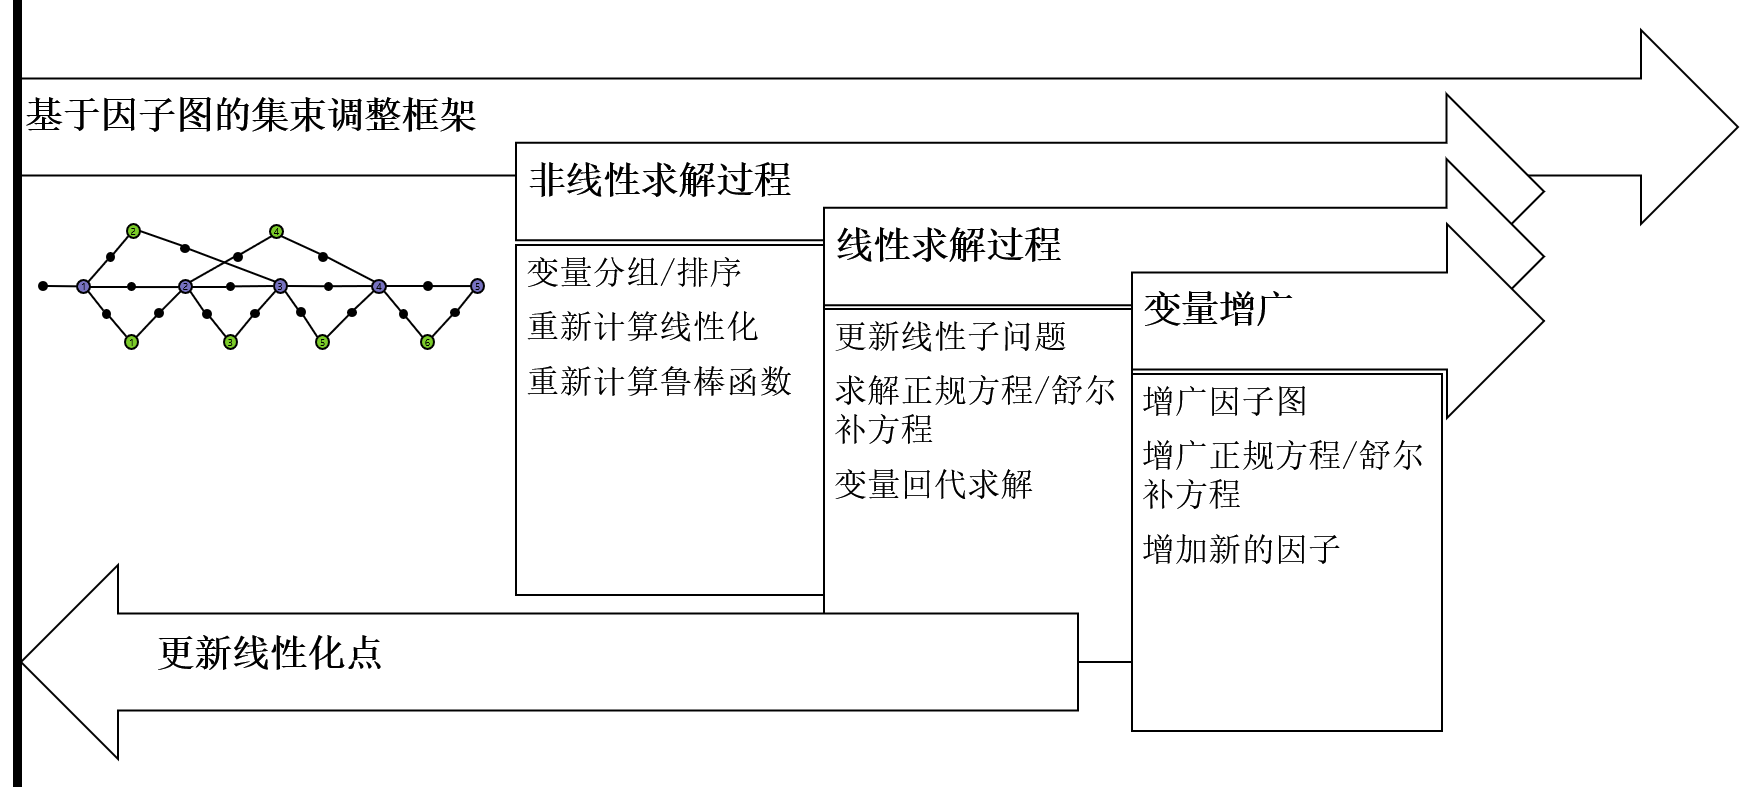
\includegraphics[scale=.5]{Pictures/framework.png}
    \caption{通用增量式集束调整框架}
    \label{fig:pipeline}
\end{figure}

\chapter{课题计划进度和预期成果}

论文的研究计划如下:
\begin{enumerate}
    \item
    资料收集和论文阅读阶段,确定本课题的具体实现细节 \\
    时间:2018.9-2018.10
    \item
    系统编码及调试阶段 \\
    时间:2018.10-2018.12
    \item
    系统性能优化阶段 \\
    时间:2018.12-2019.1
    \item
    论文撰写阶段 \\
    时间:2018.12-2019.1
\end{enumerate}

\ZJUbackmatter
\ZJUthesisbib{proposalbib.bib}

\end{document}
